\documentclass[11pt,a4paper]{article}
\usepackage[utf8]{inputenc}
\usepackage[T1]{fontenc}
\usepackage[spanish,es-noshorthands]{babel}
\usepackage{amsmath,amssymb,amsthm}
\usepackage{bm}
\usepackage{geometry}
\geometry{margin=2.5cm}
\usepackage{graphicx}
\graphicspath{{../figuras/}}
\usepackage{float}
\usepackage{xcolor}
\usepackage{hyperref}
\hypersetup{colorlinks=true,linkcolor=blue!50!black,citecolor=blue!50!black,urlcolor=blue!50!black}
\usepackage{enumitem}
\usepackage{booktabs}
\newtheorem{definition}{Definición}
\newtheorem{remark}{Observación}
\newcommand{\R}{\mathbb{R}}
\newcommand{\thetavec}{\bm{\theta}}
\newcommand{\transp}{^{\top}}
\newcommand{\promptIA}[1]{\begin{center}\fcolorbox{gray}{gray!8}{\parbox{0.9\linewidth}{\small\textbf{[FIGURA -- PROMPT IA]}\\[2pt]#1}}\end{center}}
\title{\textbf{La neurona, la sinapsis y la tasa de disparo}\\[2pt]\large Del hardware celular a la variable que modela Wilson--Cowan}
\author{Proyecto Wilson--Cowan --- Iniciación a la I+D ITBA}
\date{\today}
\begin{document}
\maketitle
\tableofcontents
\bigskip

\section*{Por qué este documento}
\addcontentsline{toc}{section}{Por qué este documento}

El modelo de Wilson--Cowan (WC) no habla de neuronas: habla de \emph{tasas de
disparo} de dos poblaciones, una excitatoria ($E$) y una inhibitoria ($I$).
Antes de meternos en las ecuaciones (ver B3, el modelo de Wilson--Cowan)
conviene entender de dónde sale esa variable y por qué es legítimo tirar a la
basura el detalle celular. Este documento es el puente: arranca en la neurona
individual, pasa por la sinapsis y termina justificando dos decisiones del
proyecto que después damos por sentadas: (i) que la variable de estado sea una
\emph{tasa} y no un voltaje, y (ii) que la no linealidad del modelo sea una
\textbf{sigmoidea}. Como sos TA de Biología, la parte celular va rápido; el foco
está en la conexión con el modelo.

\section{La neurona: soma, dendritas, axón y potencial de acción}

\subsection*{Anatomía funcional, en tres partes}
Una neurona típica tiene tres regiones con roles distintos:
\begin{itemize}[nosep]
  \item \textbf{Dendritas}: el árbol de entrada. Reciben señales de otras
  neuronas y las conducen hacia el cuerpo celular.
  \item \textbf{Soma} (cuerpo celular): integra todas esas entradas. Contiene el
  núcleo y la maquinaria metabólica.
  \item \textbf{Axón}: la salida. Un cable único (a veces largo, hasta un metro)
  que transmite la señal a las neuronas siguientes. Empieza en el
  \emph{cono axónico}, la zona donde se decide si la neurona dispara o no.
\end{itemize}

\promptIA{Ilustración anatómica científica, estilo libro de texto de
neurociencia (limpio, fondo blanco, colores planos suaves). Una neurona
piramidal vista de perfil, con etiquetas en español apuntando a: dendritas
(árbol ramificado arriba), soma o cuerpo celular (con el núcleo visible), cono
axónico (transición soma--axón), axón (cable largo hacia abajo), vaina de
mielina (segmentos), nódulos de Ranvier, y terminales axónicas (botones
sinápticos al final). Flechas finas que indiquen el sentido del flujo de
información: dendritas $\rightarrow$ soma $\rightarrow$ axón $\rightarrow$
terminales. Tipografía sans-serif, aspecto de figura de Kandel. Proporción
apaisada.}

\subsection*{Potencial de membrana y potencial de acción}
En reposo la membrana está polarizada: el interior es negativo respecto del
exterior, con un \emph{potencial de reposo} de alrededor de $-65$ mV,
sostenido por gradientes iónicos (sobre todo Na$^+$ y K$^+$) y bombas activas.
Las entradas sinápticas empujan ese potencial hacia arriba (despolarizan) o
hacia abajo (hiperpolarizan). El soma \textbf{integra} esas empujadas.

Si la despolarización en el cono axónico supera un \textbf{umbral}
(típicamente $\sim -55$ mV), se dispara un \textbf{potencial de acción} o
\emph{spike}: una excursión rápida y estereotipada del voltaje (sube a
$\sim +30$ mV y vuelve a bajar en $\sim 1$--$2$ ms), seguida de un
\emph{período refractario} durante el cual no puede dispararse otro. La clave
para lo que sigue: el spike es \textbf{todo-o-nada}. No codifica información en
su amplitud (siempre es igual), sino en \emph{cuándo} y \emph{con qué
frecuencia} ocurre. Esta observación es la semilla de la Sección~\ref{sec:rate}.

\begin{figure}[H]\centering
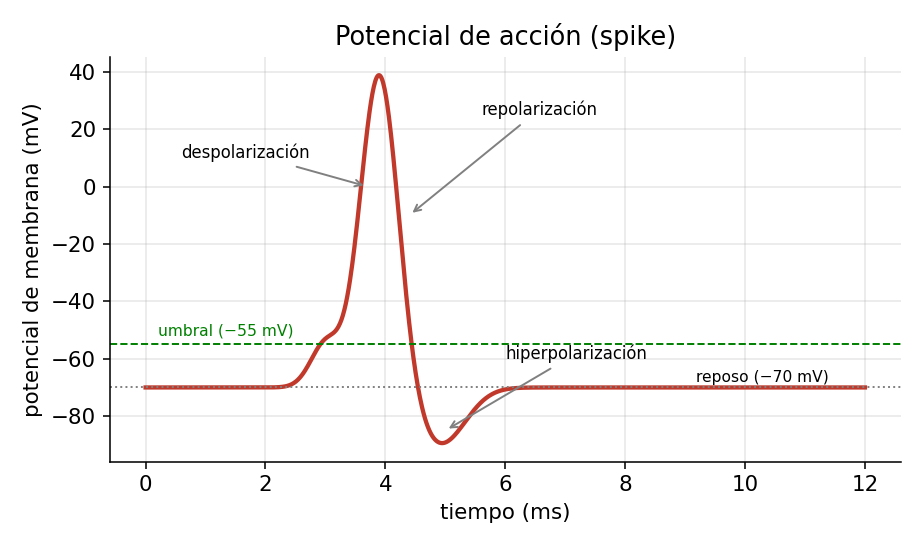
\includegraphics[width=0.62\linewidth]{fig_potencial_accion.png}
\caption{Esquema del potencial de acción: desde el reposo ($-70$~mV), la despolarización cruza el umbral ($-55$~mV), dispara un pico agudo, y sigue la repolarización y una breve hiperpolarización antes de volver al reposo.}
\end{figure}

\section{La sinapsis: cómo se comunican dos neuronas}

Cuando un spike llega a la terminal axónica, hay que pasar la señal a la
neurona siguiente. En la sinapsis química ---la dominante en el cerebro--- eso
ocurre así: el spike abre canales de Ca$^{2+}$, entra calcio, y eso gatilla la
liberación de \textbf{neurotransmisores} desde vesículas hacia la
\emph{hendidura sináptica}. Esas moléculas cruzan el espacio, se unen a
receptores en la neurona \emph{postsináptica} y abren canales iónicos que
cambian su potencial de membrana.

El \textbf{signo} del efecto depende del par neurotransmisor--receptor, y esta
distinción es exactamente la que WC hereda:
\begin{itemize}[nosep]
  \item \textbf{Excitatoria}: despolariza a la postsináptica (la acerca al
  umbral, la hace \emph{más} propensa a disparar). El neurotransmisor
  excitatorio por excelencia en el cortex es el \textbf{glutamato}.
  \item \textbf{Inhibitoria}: hiperpolariza (la aleja del umbral, la hace
  \emph{menos} propensa a disparar). El inhibitorio principal es el
  \textbf{GABA} ($\gamma$-aminobutírico).
\end{itemize}

\begin{remark}
Una simplificación operativa que usamos en todo el proyecto: cada neurona es
``excitatoria'' o ``inhibitoria'' según el efecto que ejerce sobre sus blancos
(principio de Dale, en su versión práctica). Esto justifica partir la red en
\emph{dos} poblaciones, $E$ e $I$, cada una con un signo definido. Los cuatro
pesos de WC ($w_{EE}, w_{EI}, w_{IE}, w_{II}$) no son otra cosa que la fuerza
sináptica agregada de cada camino entre poblaciones (ver B3 y la
figura \texttt{fig\_red\_EI}).
\end{remark}

\promptIA{Ilustración científica de una sinapsis química, tipo esquema de
libro de texto. A la izquierda, la terminal axónica presináptica con vesículas
(círculos pequeños con puntos adentro = neurotransmisores) fusionándose con la
membrana. En el medio, la hendidura sináptica con moléculas de neurotransmisor
difundiendo. A la derecha, la membrana postsináptica con receptores (canales)
donde se acoplan las moléculas, y una flecha ``$\pm$'' indicando cambio de
potencial. Etiquetas en español: ``terminal presináptica'', ``vesículas'',
``neurotransmisor'', ``hendidura sináptica'', ``receptor postsináptico'',
``canal iónico''. Incluir un recuadro pequeño que contraste
``glutamato $\rightarrow$ excitación (+)'' y ``GABA $\rightarrow$ inhibición
($-$)''. Estilo plano, colores suaves, fondo blanco.}

\section{De spikes a tasa de disparo}
\label{sec:rate}

Ya dijimos que el spike es todo-o-nada: la información no está en su forma sino
en su \emph{tempo}. La forma natural de resumir esa actividad es la
\textbf{tasa de disparo} (\emph{firing rate}).

\begin{definition}[Tasa de disparo]
Número de spikes por unidad de tiempo. Se puede estimar de dos maneras
complementarias:
\begin{itemize}[nosep]
  \item \textbf{Promedio temporal}: para \emph{una} neurona, contar spikes en
  una ventana $\Delta t$ y dividir por $\Delta t$. Requiere que la señal sea
  aproximadamente estacionaria en esa ventana.
  \item \textbf{Promedio poblacional}: en \emph{un} instante, contar cuántas
  neuronas de un grupo disparan y dividir por el tamaño del grupo (y por
  $\Delta t$). No necesita estacionariedad; captura la actividad
  \emph{instantánea} de la población.
\end{itemize}
\end{definition}

Para WC nos interesa el segundo: la variable $E(t)$ es la fracción (o tasa
normalizada) de neuronas excitatorias activas cerca del instante $t$, e $I(t)$
lo mismo para las inhibitorias. Pasar de un tren de spikes discreto a una tasa
continua tiene tres ventajas decisivas para este proyecto:

\begin{enumerate}[nosep]
  \item \textbf{Es una variable continua y suave.} Los spikes son eventos
  discretos y no diferenciables; una tasa promediada es una función suave de
  $t$. Eso es lo que permite escribir \emph{ecuaciones diferenciales}
  (ver M2, EDOs y sistemas dinámicos) y, más adelante, entrenar una
  \emph{Neural ODE} sobre ella (ver P4).
  \item \textbf{Es lo que realmente se mide.} Las técnicas macroscópicas
  ---EEG, LFP, fMRI, imaging de calcio--- no ven spikes individuales: ven
  actividad \emph{agregada} de miles o millones de neuronas. La tasa
  poblacional es la variable observable, no una comodidad matemática.
  \item \textbf{Promedia el ruido.} Un spike individual es ruidoso e
  impredecible; el promedio sobre una población es mucho más reproducible. Esto
  conecta con el planteo de identificación del proyecto, donde partimos de
  datos sintéticos \emph{con ruido} y aun así queremos recuperar parámetros.
\end{enumerate}

\section{La curva f--I y por qué la sigmoidea}
\label{sec:fi}

Falta el ingrediente que cierra el puente: ¿cómo depende la tasa de disparo de
la \emph{entrada} que recibe la neurona (o la población)? La respuesta empírica
es la \textbf{curva f--I} (frecuencia de disparo $f$ vs.\ corriente de entrada
$I_{\text{ent}}$), y su forma es la razón de ser de la sigmoidea de WC.

\subsection*{Forma de la curva f--I: umbral y saturación}
Medí experimentalmente la frecuencia de disparo de una neurona (o el promedio
de una población) en función de la corriente inyectada. Obtenés una curva con
tres regímenes:
\begin{enumerate}[nosep]
  \item \textbf{Zona subumbral}: con poca entrada, la neurona no llega al
  umbral y \emph{no dispara}. La tasa es $\approx 0$. Ver acá la traducción de
  la Sección~1: el umbral del potencial de acción reaparece como el
  ``pie'' plano de la curva.
  \item \textbf{Zona de crecimiento}: pasado el umbral, más entrada
  $\Rightarrow$ más frecuencia, de forma aproximadamente monótona.
  \item \textbf{Zona de saturación}: por el período refractario, hay un tope
  físico a cuántos spikes por segundo se pueden emitir. Por más que subas la
  entrada, la tasa se aplana en un máximo.
\end{enumerate}
Umbral abajo, saturación arriba, crecimiento monótono en el medio: eso es,
cualitativamente, una \textbf{S} ---una \emph{sigmoidea}.

\subsection*{La abstracción que usa Wilson--Cowan}
WC no modela la curva f--I de \emph{una} neurona, sino la \textbf{respuesta
media de una población}: qué fracción de la población dispara dado un nivel de
entrada agregado. Ese promateado sobre muchas neuronas con umbrales
ligeramente distintos suaviza los codos y produce una sigmoidea limpia. WC la
escribe como una función logística:
\begin{equation}
  S_a(u) \;=\; \frac{1}{1+e^{-a\,u}},
  \label{eq:sigmoid}
\end{equation}
donde $u$ es la entrada neta a la población y $a$ es la \textbf{ganancia}: qué
tan abrupta es la transición de ``apagado'' a ``encendido''. La
Figura~\ref{fig:sigmoidea} muestra las sigmoideas de $E$ e $I$ tal como se usan
en el simulador.

\begin{figure}[H]
  \centering
  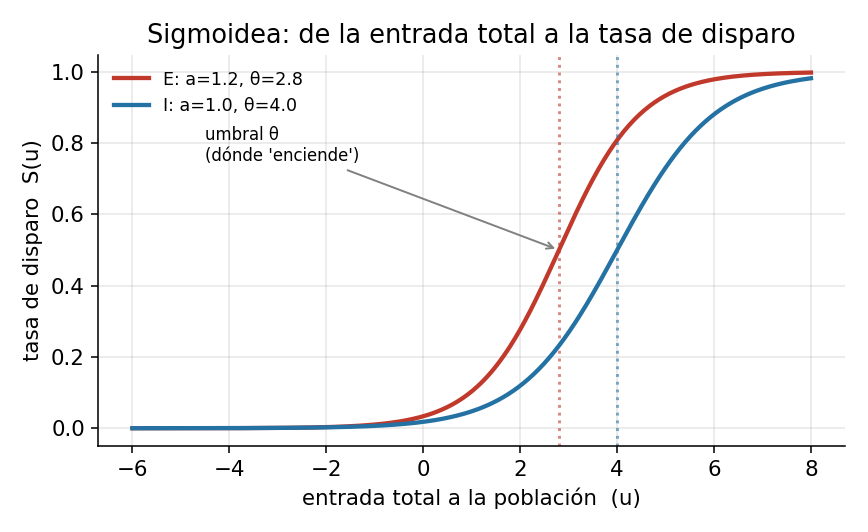
\includegraphics[width=0.75\linewidth]{fig_sigmoidea.png}
  \caption{Función sigmoidea $S_a(u)=1/(1+e^{-au})$ para las poblaciones $E$ e
  $I$, con su umbral. Es la abstracción de la curva f--I: pie plano
  (subumbral), crecimiento monótono y saturación en 1. Es la única no
  linealidad del modelo. (figura del proyecto)}
  \label{fig:sigmoidea}
\end{figure}

\begin{remark}[Dónde entran los 10 parámetros]
La forma \eqref{eq:sigmoid} de la sigmoidea aparece dentro de las dos ecuaciones
de WC (ver B3). La entrada neta $u$ de cada población es una combinación pesada
de las actividades más el estímulo externo y un umbral; por ejemplo, para la
población excitatoria, $u = w_{EE}E - w_{EI}I + P(t) - \theta_e$. Ahí viven
varios de los diez parámetros del proyecto:
\begin{itemize}[nosep]
  \item la \textbf{ganancia} $a$ de \eqref{eq:sigmoid} son los parámetros
  $a_e=1.2$, $a_i=1.0$ (qué tan abrupta es la S de cada población);
  \item el \textbf{umbral} de la curva f--I son $\theta_e=2.8$, $\theta_i=4.0$
  (dónde está el ``pie'' de la S, es decir cuánta entrada hace falta para
  empezar a disparar);
  \item los \textbf{pesos} $w_{EE}=6.4$, $w_{EI}=4.8$, $w_{IE}=6.0$,
  $w_{II}=1.2$ pesan cuánto se activan/frenan las poblaciones entre sí ---son la
  fuerza sináptica agregada de la Sección~2;
  \item las \textbf{constantes de tiempo} $\tau_e=1.0$, $\tau_i=2.0$ fijan qué
  tan rápido cada población relaja hacia su tasa de equilibrio.
\end{itemize}
En el modelo también aparecen los \emph{offsets} $k_e, k_i$, pero no son
parámetros libres: se derivan de $a$ y $\theta$ para que el reposo $E=I=0$ sea
un equilibrio sin estímulo (ver B3). Entre esos diez, $w_{II}$ es el que después
resulta difícil de identificar; es el hilo conductor de todo el paquete.
\end{remark}

\section{Por qué modelar poblaciones y no neuronas}

Con todo lo anterior en la mano, la decisión de fondo del proyecto se explica
sola. Podríamos, en principio, simular cada neurona con su voltaje, sus canales
y sus spikes (modelos tipo Hodgkin--Huxley o integrate-and-fire). ¿Por qué no lo
hacemos?

\begin{itemize}
  \item \textbf{Escala y dimensionalidad.} Un pedacito de cortex tiene
  $\sim 10^5$--$10^6$ neuronas y órdenes de magnitud más sinapsis. Un modelo
  neurona-por-neurona tiene millones de variables de estado y muchísimos más
  parámetros. Es intratable de simular, imposible de analizar y sin esperanza
  de \emph{identificar} desde datos. WC colapsa todo eso a \textbf{dos}
  variables, $E(t)$ e $I(t)$, y \textbf{diez} parámetros. Esa reducción es lo
  que hace viable el diagnóstico de identificabilidad con Fisher$+$SVD que es el
  corazón del proyecto.
  \item \textbf{Lo que se mide es agregado.} Como vimos en la
  Sección~\ref{sec:rate}, las señales experimentales (EEG, LFP, fMRI) reflejan
  actividad de poblaciones, no de neuronas sueltas. Modelar en la variable que
  efectivamente se observa es lo honesto: no tiene sentido pelear por
  identificar estados que ningún instrumento ve.
  \item \textbf{Los fenómenos de interés son colectivos.} Las oscilaciones que
  nos importan ---el régimen \emph{theta-gamma} objetivo del proyecto--- son
  ritmos de \emph{población}. Emergen de la interacción $E$--$I$ (un ciclo
  límite; ver M2 y B3), no de una neurona aislada. La variable poblacional es la
  escala donde el fenómeno \emph{existe}.
\end{itemize}

Esta es la idea de \emph{modelo de masa neuronal} (\emph{neural mass model}):
describir la dinámica media de una población en vez del detalle celular.
Wilson--Cowan (1972, 1973) es el ejemplo fundacional. En B2 formalizamos el paso
``de muchas neuronas ruidosas a dos tasas suaves''; en B3 escribimos las
ecuaciones completas y mostramos que con los valores de la tabla el sistema
oscila. Con este documento cerrado, ya tenés la traducción biológica de las dos
piezas centrales: la \emph{variable} (tasa de disparo poblacional) y la
\emph{no linealidad} (sigmoidea, heredera directa de la curva f--I).

\begin{thebibliography}{9}
\bibitem{kandel} E.~R. Kandel, J.~H. Schwartz, T.~M. Jessell, S.~A. Siegelbaum,
A.~J. Hudspeth, \emph{Principles of Neural Science}, 5\textsuperscript{a} ed.,
McGraw-Hill, 2013.
\bibitem{dayan} P.~Dayan, L.~F. Abbott, \emph{Theoretical Neuroscience:
Computational and Mathematical Modeling of Neural Systems}, MIT Press, 2001.
\bibitem{gerstner} W.~Gerstner, W.~M. Kistler, R.~Naud, L.~Paninski,
\emph{Neuronal Dynamics: From Single Neurons to Networks and Models of
Cognition}, Cambridge University Press, 2014.
\bibitem{wc1972} H.~R. Wilson, J.~D. Cowan, ``Excitatory and inhibitory
interactions in localized populations of model neurons'', \emph{Biophysical
Journal} 12(1):1--24, 1972.
\bibitem{wc1973} H.~R. Wilson, J.~D. Cowan, ``A mathematical theory of the
functional dynamics of cortical and thalamic nervous tissue'', \emph{Kybernetik}
13:55--80, 1973.
\end{thebibliography}

\end{document}
